\documentclass[11pt,twocolumn,letterpaper]{article}
\usepackage{lipsum, babel}

\usepackage{times}
\usepackage{epsfig}
\usepackage{graphicx}
\usepackage{amsmath}
\usepackage{amssymb}

\usepackage{url}
% Include other packages here, before hyperref.

% If you comment hyperref and then uncomment it, you should delete
% egpaper.aux before re-running latex.  (Or just hit 'q' on the first latex
% run, let it finish, and you should be clear).
\usepackage[pagebackref=true,breaklinks=true,letterpaper=true,colorlinks,bookmarks=false]{hyperref}

% \cvprfinalcopy % *** Uncomment this line for the final submission
\newcommand*{\imouse}{
\includegraphics[scale=0.03]{fig1/mouse1.png}}
\newcommand*{\iphone}{
\includegraphics[scale=0.06]{fig1/microphone.png}}

%\def\cvprPaperID{326} % *** Enter the CVPR Paper ID here
%\def\httilde{\mbox{\tt\raisebox{-.5ex}{\symbol{126}}}}

% Pages are numbered in submission mode, and unnumbered in camera-ready
%\ifcvprfinal\pagestyle{empty}\fi
\begin{document}
\onecolumn

%%%%%%%%% TITLE
\title{ Draw\&Tell: Efficient Annotation for Semantic Image Segmentation via Drawing and Speaking}

\maketitle
%\thispagestyle{empty}

%%%%%%%%% ABSTRACT

In this supplementary material, we present 1) the interface of our annotation tool Draw\&Tell and 2) exemplar annotations by Draw\&Tell. In order to boost research in this direction, we will release the code of Draw\&Tell and all the annotated images.

%%%%%%%%% BODY TEXT
\section{Interface}
Please see Fig.~\ref{fig:0} for the interface of our annotation tool Draw\&Tell. 
Annotators can draw scribbles on objects of interest and speak their names in the meanwhile. The name of the object is obtained by the combination of speech recognition and webly-supervised object recognition. The recognized object name is displayed right after the drawing of the scribbles. The names of all the classes of interest are shown at the bottom for reference. 

Annotators are allowed to draw multiple scribbles for the same object, as shown in Fig.~\ref{fig:0} by the horse example. In this case, the annotator only needs to speak for the first scribble. The subsequent scribbles are grouped to the first one -- the most recent scribble with \emph{successful} name recognition -- if \emph{silence} is detected for them by the speech recognition engine. 


\begin{figure*}
\centering
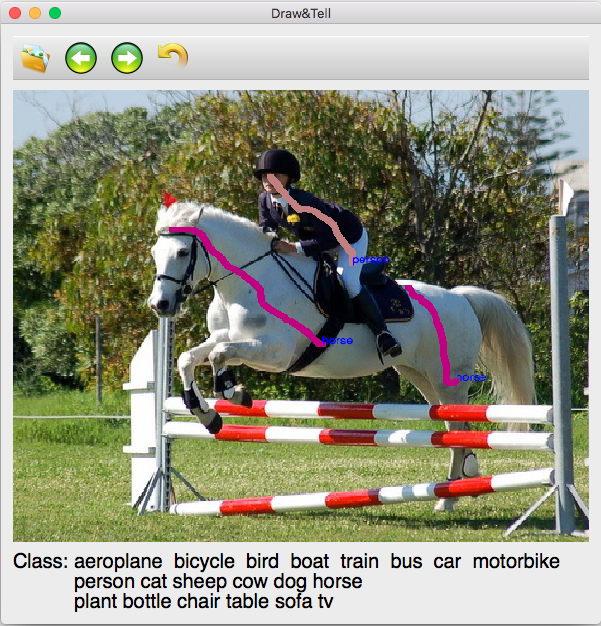
\includegraphics[width=0.7\linewidth]{figSM/draw_tell_interface.png} 
\caption{The interface of Draw\&Tell.  Annotators can draw scribbles on objects of interest and speak their names in the meanwhile. The names of all the classes of interest are shown at the bottom for reference. The names of the object are obtained by speech recognition and are shown right after the drawing of the scribbles. Annotators can correct the result if it is wrong.}
\label{fig:0}
\end{figure*}


\section{Annotation Examples}
In this section, we show annotation examples via our annotation tool Draw\&Tell, together with that of other two typical annotations.
In total, we show four forms of annotations: 
(a) full segmentation masks, (b) bounding boxes, (c) semantic scribbles by Anno-1.5 (Draw\&Tell on a budget of 1.5 seconds per object), and (d) semantic scribbles by Anno-3 (Draw\&Tell on a budget of 3 seconds per object).  Please see Fig.~\ref{fig:1} to Fig.~\ref{fig:12} for some sampled examples. The annotation tool Draw\&Tell and all the annotations will be released. 

\begin{figure*} 
$\begin{tabular}{ccccc}
\hspace{-2mm}
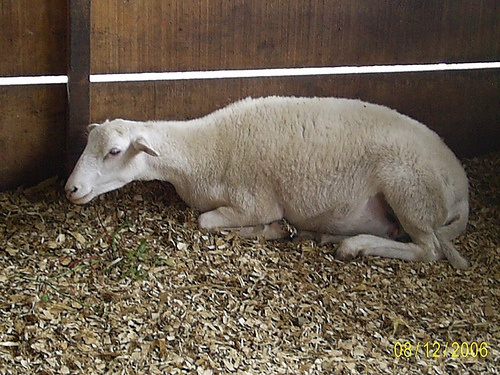
\includegraphics[width=0.48\linewidth]{figSM/2007_000676.jpg} & 
 \\
 \hspace{-2mm}  
\footnotesize{\text{ input image }} &  \\ 
\hspace{-2mm}
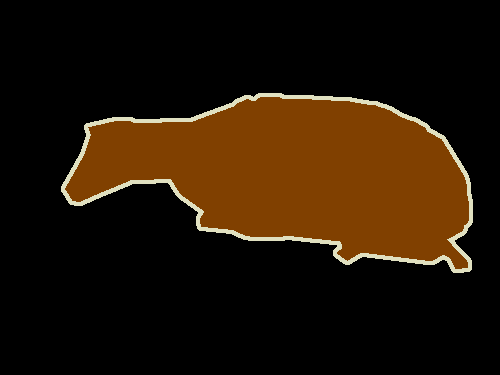
\includegraphics[width=0.48\linewidth]{figSM/2007_000676_gt.png} &
\hspace{-4mm} 
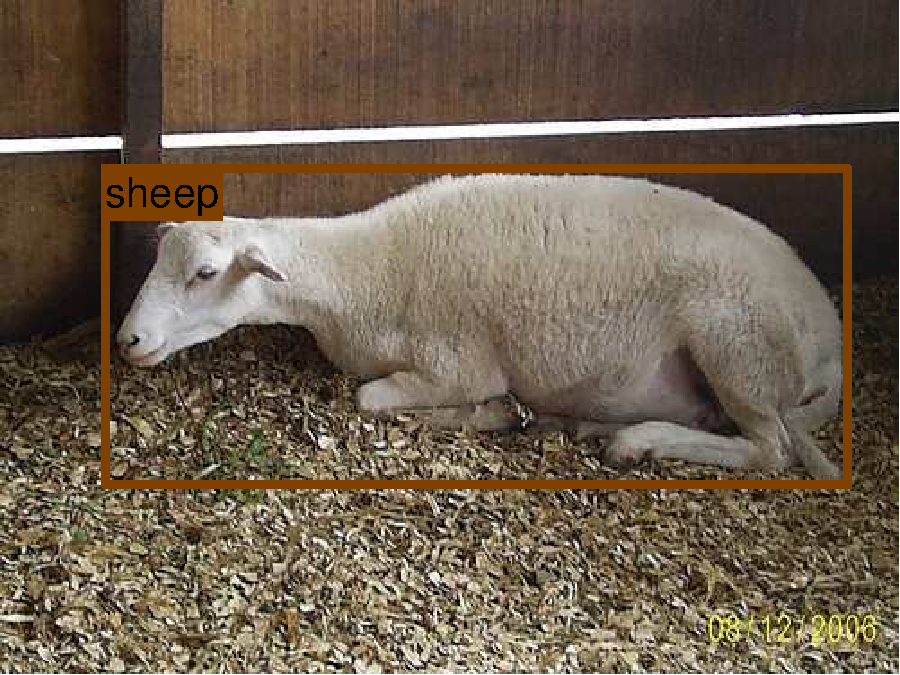
\includegraphics[width=0.48\linewidth]{figSM/2007_000676_bbx-crop.pdf} \\
\hspace{-2mm}  
\footnotesize{\text{(a) full segmentation mask }} & 
 \hspace{-4mm} 
\footnotesize{\text{(b) bounding box}} \\ 
\hspace{-2mm} 
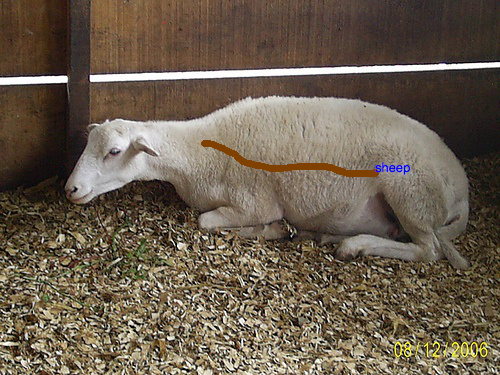
\includegraphics[width=0.48\linewidth]{figSM/2007_000676_anno_15.png} &
\hspace{-4mm} 
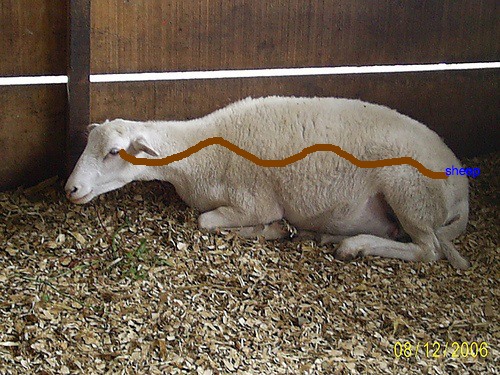
\includegraphics[width=0.48\linewidth]{figSM/2007_000676_anno_3.png}\\
\hspace{-2mm}  
\footnotesize{\text{(c) Semantic Scribbles (Anno-1.5, ours) }} & 
 \hspace{-4mm} 
\footnotesize{\text{(d) Semantic Scribbles (Anno-3, ours)}} \\ 
\end{tabular}$
\caption{A comparison of our annotations to the standard ones used for semantic segmentation. Note that our annotations are significantly cheaper to obtain, but yield comparable results. See the paper for details.}
\label{fig:1}
\end{figure*}


\begin{figure*} 
$\begin{tabular}{ccccc}
\hspace{-2mm}
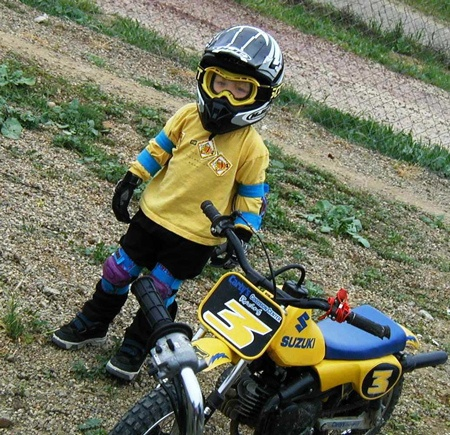
\includegraphics[width=0.48\linewidth]{figSM/2007_000733.jpg} & 
 \\
 \hspace{-2mm}  
\footnotesize{\text{ input image }} &  \\ 
\hspace{-2mm}

\includegraphics[width=0.48\linewidth]{figSM/2007_000733_gt.png} &
\hspace{-4mm} 
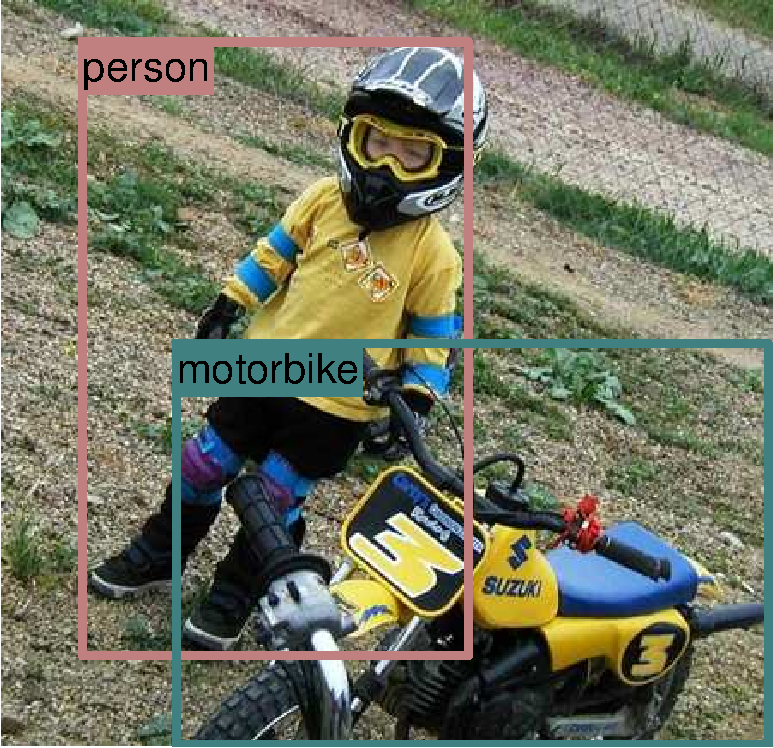
\includegraphics[width=0.48\linewidth]{figSM/2007_000733_bbx-crop.pdf} \\
\hspace{-2mm}  
\footnotesize{\text{(a) full segmentation mask }} & 
 \hspace{-4mm} 
\footnotesize{\text{(b) bounding box}} \\ 
\hspace{-2mm} 
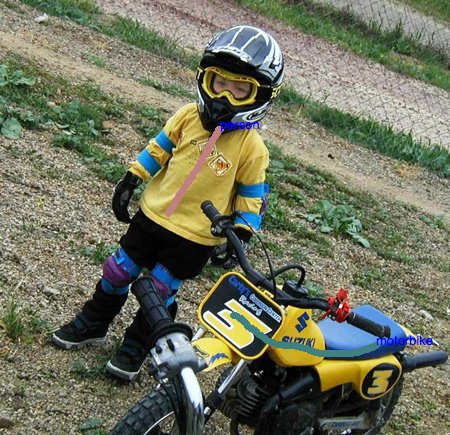
\includegraphics[width=0.48\linewidth]{figSM/2007_000733_anno_15.png} &
\hspace{-4mm} 
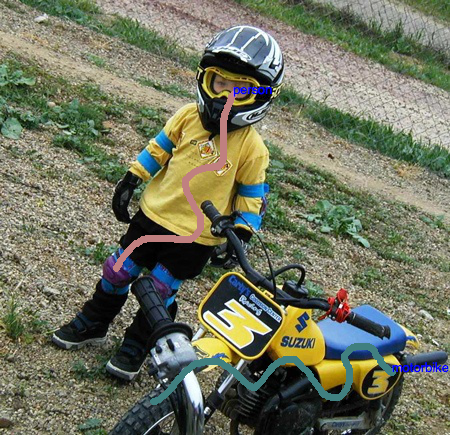
\includegraphics[width=0.48\linewidth]{figSM/2007_000733_anno_3.png}\\
\hspace{-2mm}  
\footnotesize{\text{(c) Semantic Scribbles (Anno-1.5, ours) }} & 
 \hspace{-4mm} 
\footnotesize{\text{(d) Semantic Scribbles (Anno-3, ours)}} \\ 
\end{tabular}$
\caption{A comparison of our annotations to the standard ones used for semantic segmentation. Note that our annotations are significantly cheaper to obtain, but yield comparable results. See the paper for details.}
\label{fig:2}
\end{figure*}


\begin{figure*} 
$\begin{tabular}{ccccc}
\hspace{-2mm}
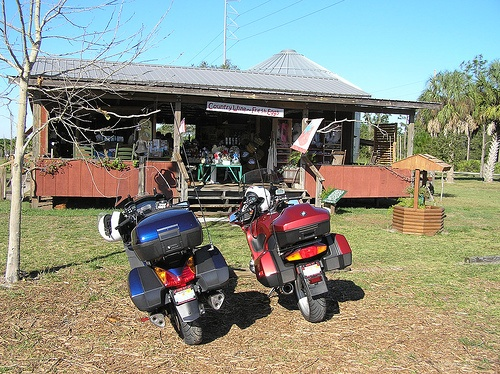
\includegraphics[width=0.48\linewidth]{figSM/2007_000822.jpg} & 
 \\
 \hspace{-2mm}  
\footnotesize{\text{ input image }} &  \\ 
\hspace{-2mm}
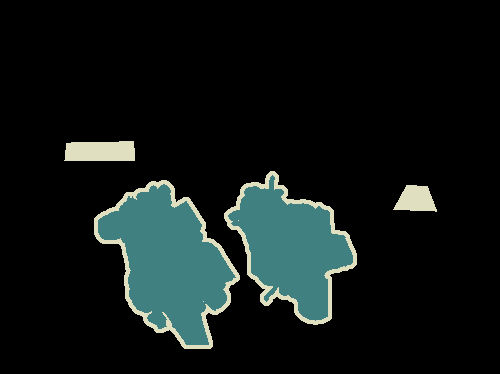
\includegraphics[width=0.48\linewidth]{figSM/2007_000822_gt.png} &
\hspace{-4mm} 
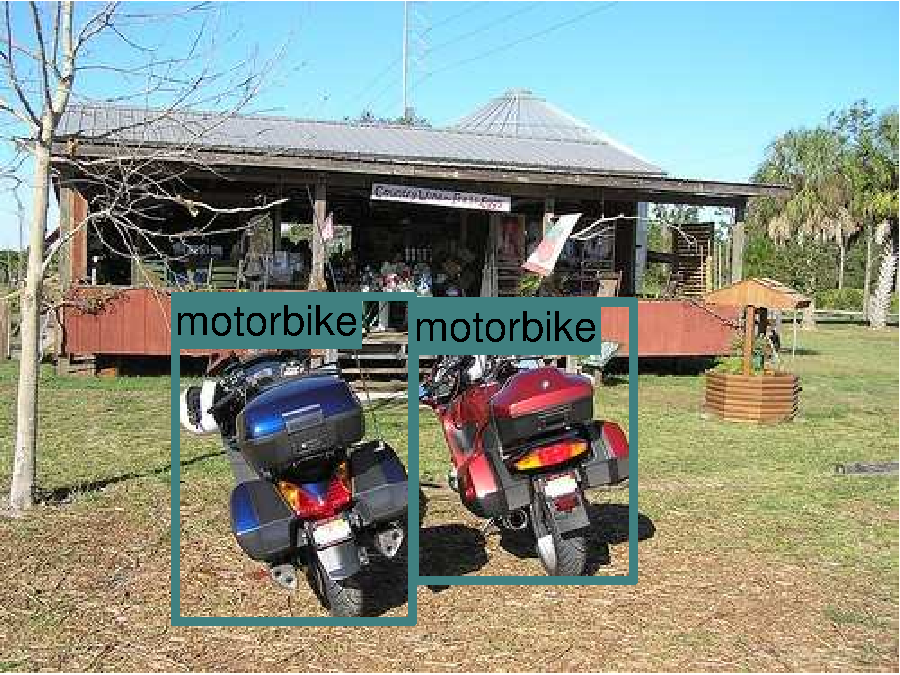
\includegraphics[width=0.48\linewidth]{figSM/2007_000822_bbx-crop.pdf} \\
\hspace{-2mm}  
\footnotesize{\text{(a) full segmentation mask }} & 
 \hspace{-4mm} 
\footnotesize{\text{(b) bounding box}} \\ 
\hspace{-2mm} 
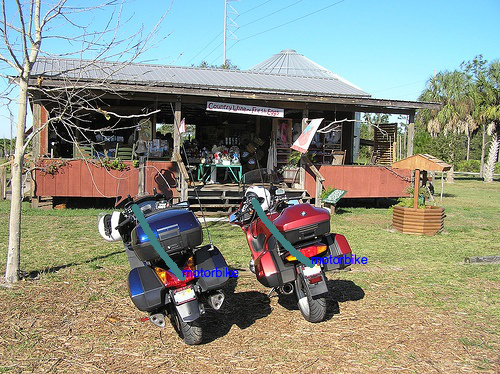
\includegraphics[width=0.48\linewidth]{figSM/2007_000822_anno_15.png} &
\hspace{-4mm} 
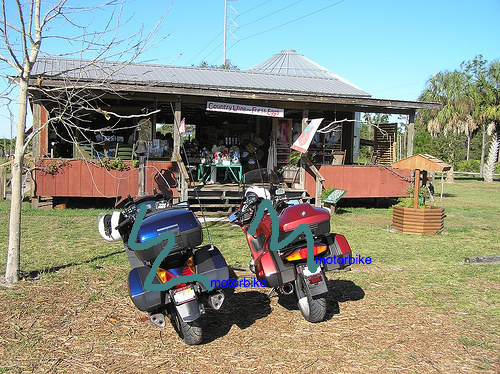
\includegraphics[width=0.48\linewidth]{figSM/2007_000822_anno_3.png}\\
\hspace{-2mm}  
\footnotesize{\text{(c) Semantic Scribbles (Anno-1.5, ours) }} & 
 \hspace{-4mm} 
\footnotesize{\text{(d) Semantic Scribbles (Anno-3, ours)}} \\ 
\end{tabular}$
\caption{A comparison of our annotations to the standard ones used for semantic segmentation. Note that our annotations are significantly cheaper to obtain, but yield comparable results. See the paper for details.}
\label{fig:3}
\end{figure*}

\begin{figure*} 
$\begin{tabular}{ccccc}
\hspace{-2mm}
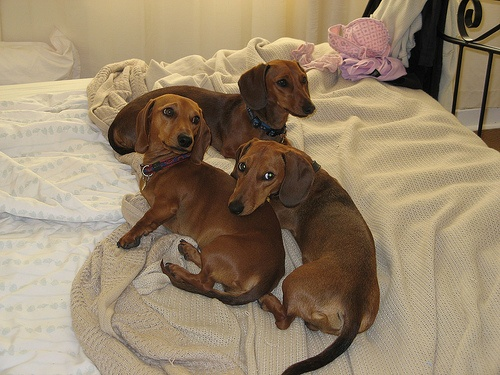
\includegraphics[width=0.48\linewidth]{figSM/2007_001239.jpg} & 
 \\
 \hspace{-2mm}  
\footnotesize{\text{ input image }} &  \\ 
\hspace{-2mm}

\includegraphics[width=0.48\linewidth]{figSM/2007_001239_gt.png} &
\hspace{-4mm} 
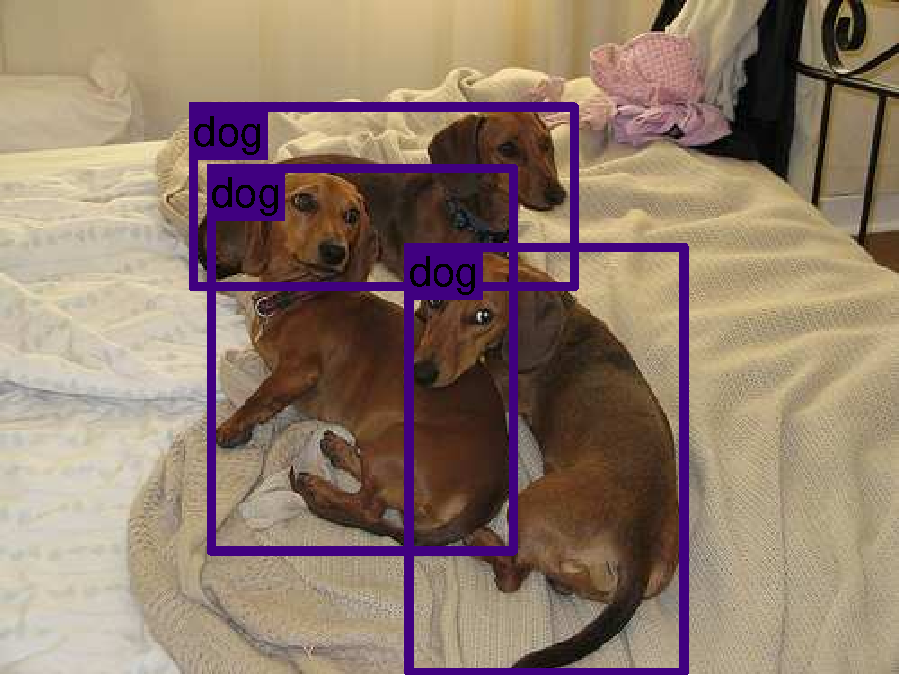
\includegraphics[width=0.48\linewidth]{figSM/2007_001239_bbx-crop.pdf} \\
\hspace{-2mm}  
\footnotesize{\text{(a) full segmentation mask }} & 
 \hspace{-4mm} 
\footnotesize{\text{(b) bounding box}} \\ 
\hspace{-2mm} 
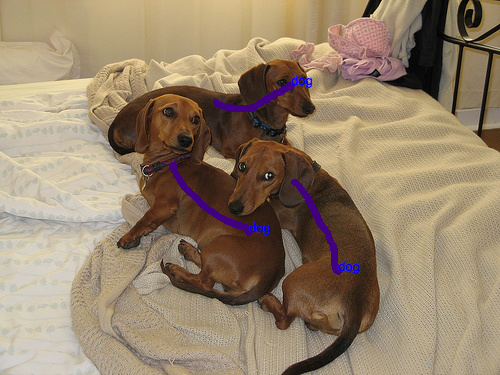
\includegraphics[width=0.48\linewidth]{figSM/2007_001239_anno_15.png} &
\hspace{-4mm} 
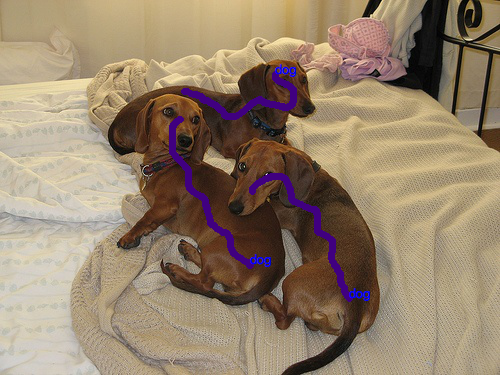
\includegraphics[width=0.48\linewidth]{figSM/2007_001239_anno_3.png}\\
\hspace{-2mm}  
\footnotesize{\text{(c) Semantic Scribbles (Anno-1.5, ours) }} & 
 \hspace{-4mm} 
\footnotesize{\text{(d) Semantic Scribbles (Anno-3, ours)}} \\ 
\end{tabular}$
\caption{A comparison of our annotations to the standard ones used for semantic segmentation. Note that our annotations are significantly cheaper to obtain, but yield comparable results. See the paper for details.}
\label{fig:4}
\end{figure*}

\begin{figure*} 
$\begin{tabular}{ccccc}
\hspace{-2mm}
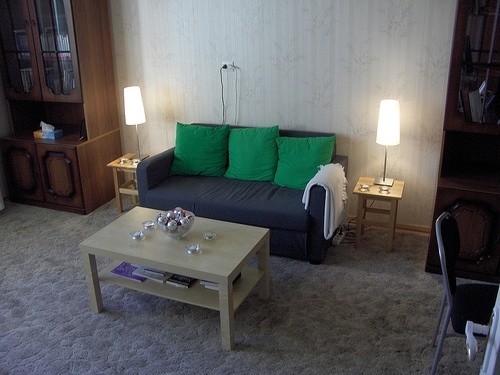
\includegraphics[width=0.48\linewidth]{figSM/2007_001457.jpg} & 
 \\
 \hspace{-2mm}  
\footnotesize{\text{ input image }} &  \\ 
\hspace{-2mm}
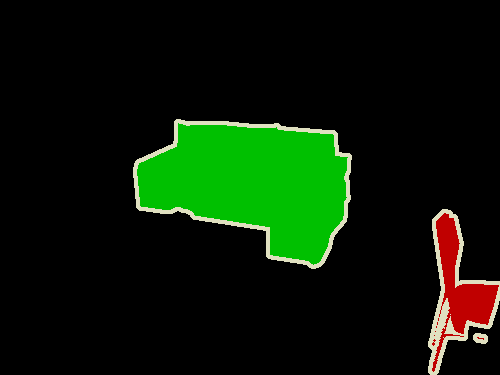
\includegraphics[width=0.48\linewidth]{figSM/2007_001457_gt.png} &
\hspace{-4mm} 
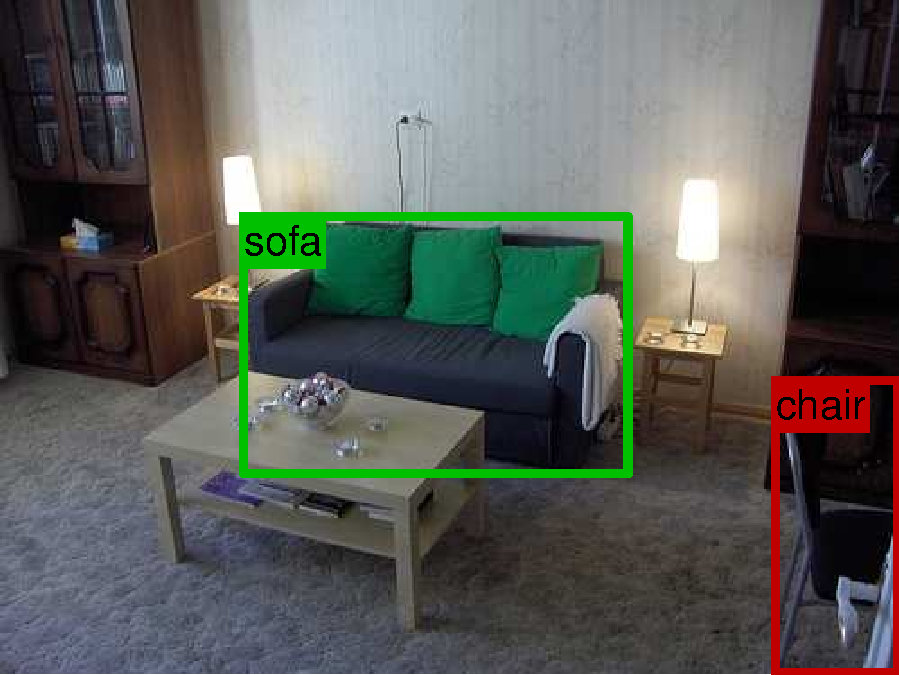
\includegraphics[width=0.48\linewidth]{figSM/2007_001457_bbx-crop.pdf} \\
\hspace{-2mm}  
\footnotesize{\text{(a) full segmentation mask }} & 
 \hspace{-4mm} 
\footnotesize{\text{(b) bounding box}} \\ 
\hspace{-2mm} 
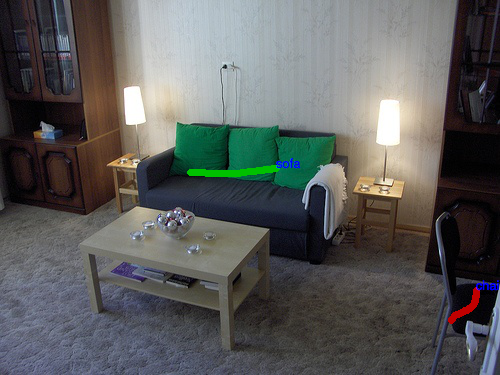
\includegraphics[width=0.48\linewidth]{figSM/2007_001457_anno_15.png} &
\hspace{-4mm} 
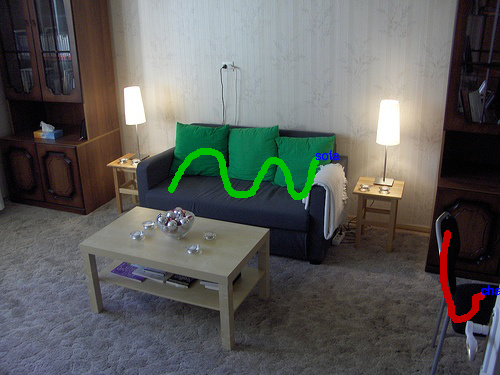
\includegraphics[width=0.48\linewidth]{figSM/2007_001457_anno_3.png}\\
\hspace{-2mm}  
\footnotesize{\text{(c) Semantic Scribbles (Anno-1.5, ours) }} & 
 \hspace{-4mm} 
\footnotesize{\text{(d) Semantic Scribbles (Anno-3, ours)}} \\ 
\end{tabular}$
\caption{A comparison of our annotations to the standard ones used for semantic segmentation. Note that our annotations are significantly cheaper to obtain, but yield comparable results. See the paper for details.}
\label{fig:5}
\end{figure*}

\begin{figure*} 
$\begin{tabular}{ccccc}
\hspace{-2mm}
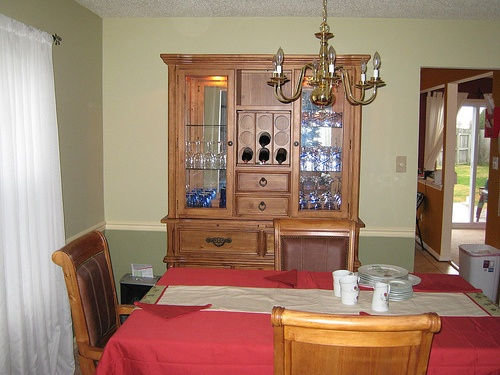
\includegraphics[width=0.48\linewidth]{figSM/2007_001677.jpg} & 
 \\
 \hspace{-2mm}  
\footnotesize{\text{ input image }} &  \\ 
\hspace{-2mm}
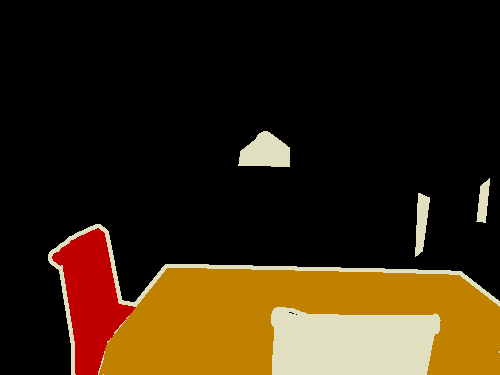
\includegraphics[width=0.48\linewidth]{figSM/2007_001677_gt.png} &
\hspace{-4mm} 
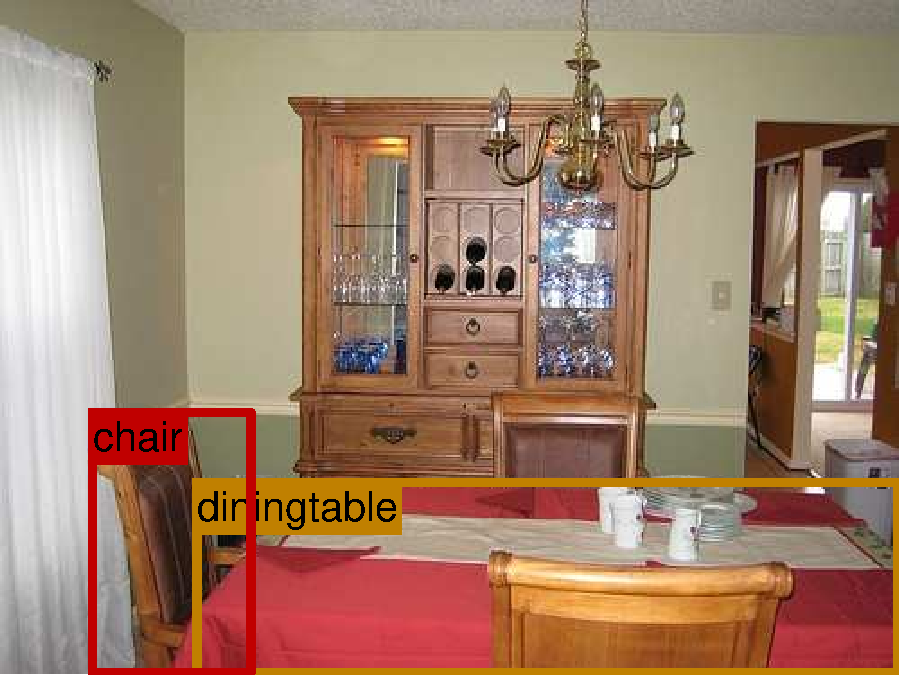
\includegraphics[width=0.48\linewidth]{figSM/2007_001677_bbx-crop.pdf} \\
\hspace{-2mm}  
\footnotesize{\text{(a) full segmentation mask }} & 
 \hspace{-4mm} 
\footnotesize{\text{(b) bounding box}} \\ 
\hspace{-2mm} 
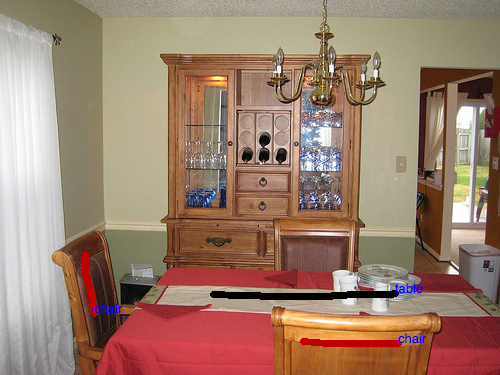
\includegraphics[width=0.48\linewidth]{figSM/2007_001677_anno_15.png} &
\hspace{-4mm} 
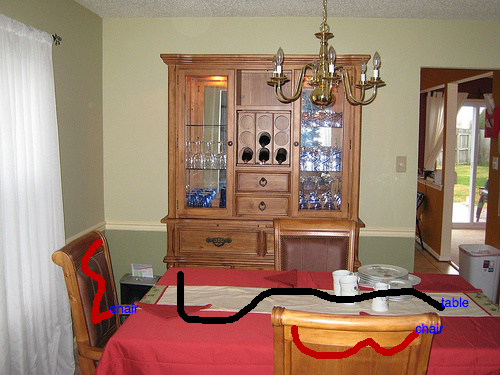
\includegraphics[width=0.48\linewidth]{figSM/2007_001677_anno_3.png}\\
\hspace{-2mm}  
\footnotesize{\text{(c) Semantic Scribbles (Anno-1.5, ours) }} & 
 \hspace{-4mm} 
\footnotesize{\text{(d) Semantic Scribbles (Anno-3, ours)}} \\ 
\end{tabular}$
\caption{A comparison of our annotations to the standard ones used for semantic segmentation. Note that our annotations are significantly cheaper to obtain, but yield comparable results. See the paper for details.}
\label{fig:6}
\end{figure*}

\begin{figure*} 
$\begin{tabular}{ccccc}
\hspace{-2mm}
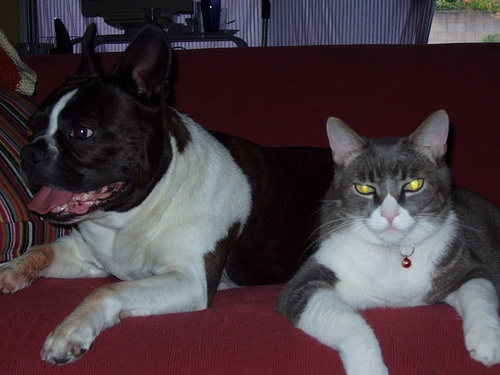
\includegraphics[width=0.48\linewidth]{figSM/2007_001763.jpg} & 
 \\
 \hspace{-2mm}  
\footnotesize{\text{ input image }} &  \\ 
\hspace{-2mm}
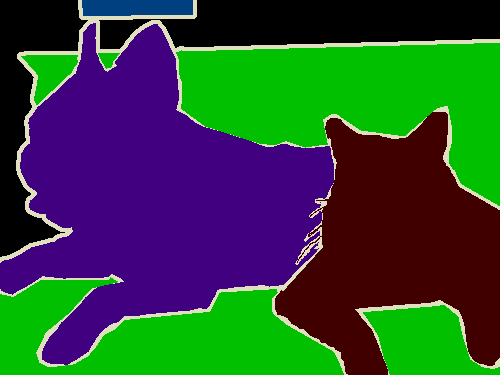
\includegraphics[width=0.48\linewidth]{figSM/2007_001763_gt.png} &
\hspace{-4mm} 
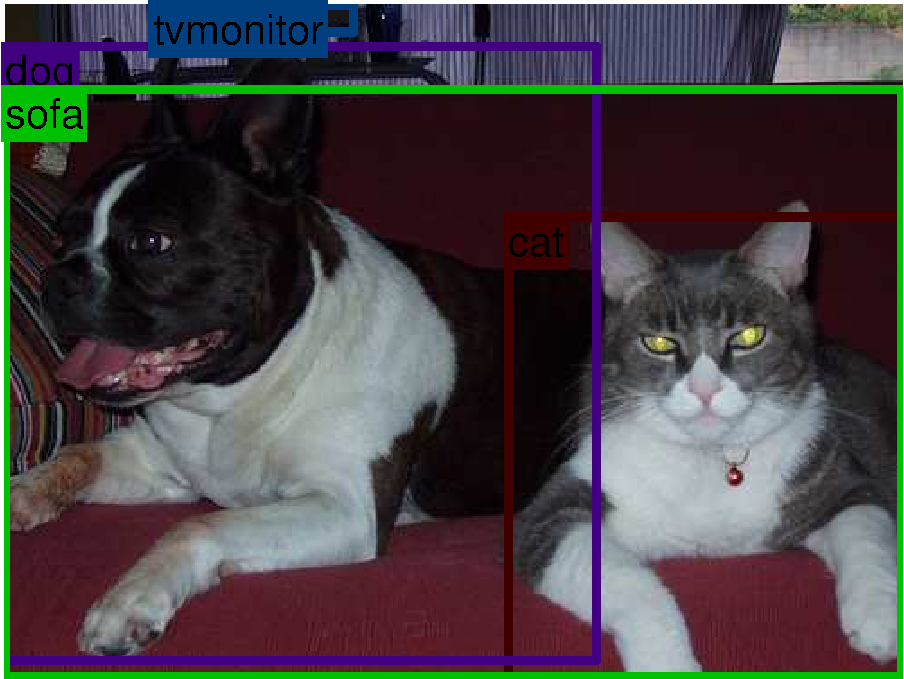
\includegraphics[width=0.48\linewidth]{figSM/2007_001763_bbx-crop.pdf} \\
\hspace{-2mm}  
\footnotesize{\text{(a) full segmentation mask }} & 
 \hspace{-4mm} 
\footnotesize{\text{(b) bounding box}} \\ 
\hspace{-2mm} 
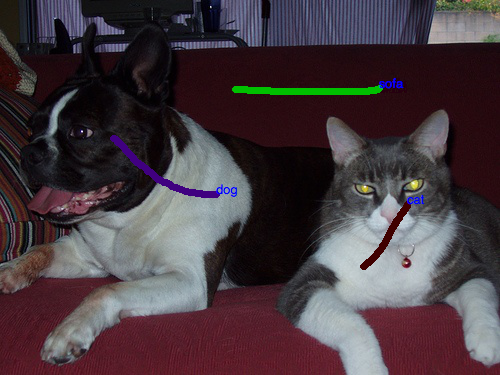
\includegraphics[width=0.48\linewidth]{figSM/2007_001763_anno_15.png} &
\hspace{-4mm} 
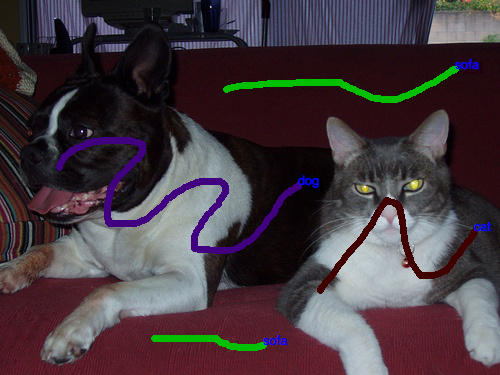
\includegraphics[width=0.48\linewidth]{figSM/2007_001763_anno_3.png}\\
\hspace{-2mm}  
\footnotesize{\text{(c) Semantic Scribbles (Anno-1.5, ours) }} & 
 \hspace{-4mm} 
\footnotesize{\text{(d) Semantic Scribbles (Anno-3, ours)}} \\ 
\end{tabular}$
\caption{A comparison of our annotations to the standard ones used for semantic segmentation. Note that our annotations are significantly cheaper to obtain, but yield comparable results. See the paper for details.}
\label{fig:7}
\end{figure*}

\begin{figure*} 
$\begin{tabular}{ccccc}
\hspace{-2mm}
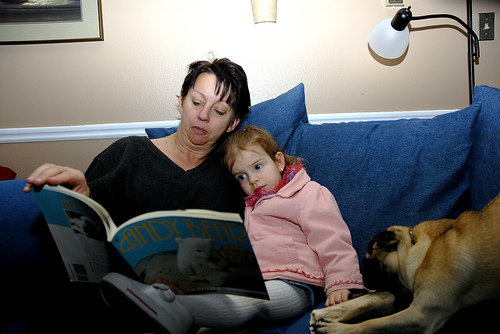
\includegraphics[width=0.48\linewidth]{figSM/2008_000270.jpg} & 
 \\
 \hspace{-2mm}  
\footnotesize{\text{ input image }} &  \\ 
\hspace{-2mm}
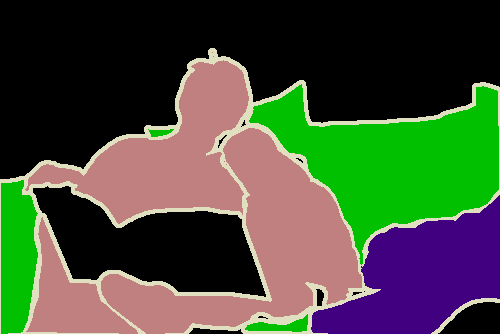
\includegraphics[width=0.48\linewidth]{figSM/2008_000270_gt.png} &
\hspace{-4mm} 
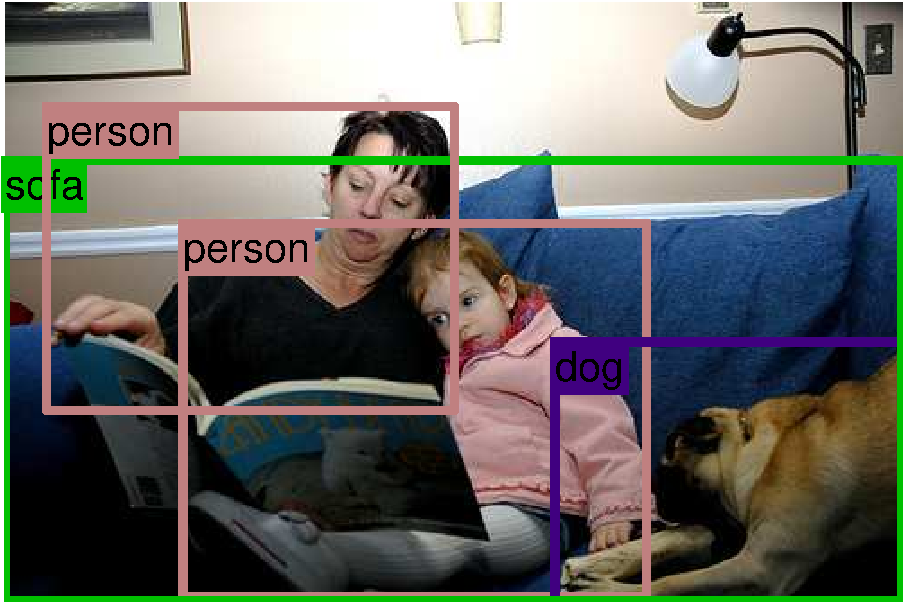
\includegraphics[width=0.48\linewidth]{figSM/2008_000270_bbx-crop.pdf} \\
\hspace{-2mm}  
\footnotesize{\text{(a) full segmentation mask }} & 
 \hspace{-4mm} 
\footnotesize{\text{(b) bounding box}} \\ 
\hspace{-2mm} 
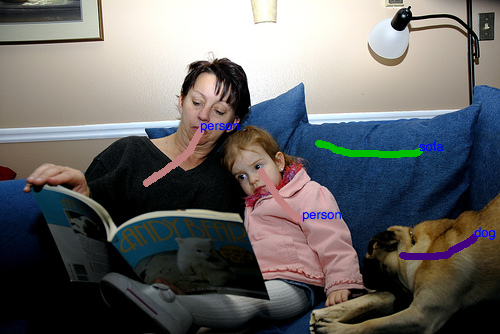
\includegraphics[width=0.48\linewidth]{figSM/2008_000270_anno_15.png} &
\hspace{-4mm} 
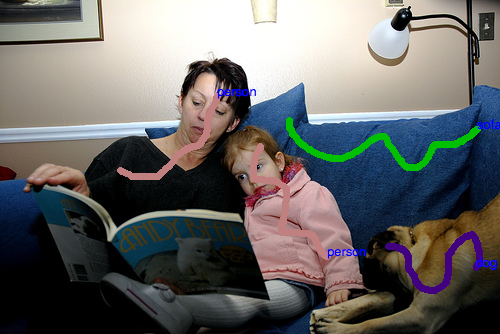
\includegraphics[width=0.48\linewidth]{figSM/2008_000270_anno_3.png}\\
\hspace{-2mm}  
\footnotesize{\text{(c) Semantic Scribbles (Anno-1.5, ours) }} & 
 \hspace{-4mm} 
\footnotesize{\text{(d) Semantic Scribbles (Anno-3, ours)}} \\ 
\end{tabular}$
\caption{A comparison of our annotations to the standard ones used for semantic segmentation. Note that our annotations are significantly cheaper to obtain, but yield comparable results. See the paper for details.}
\label{fig:8}
\end{figure*}


\begin{figure*} 
$\begin{tabular}{ccccc}
\hspace{-2mm}
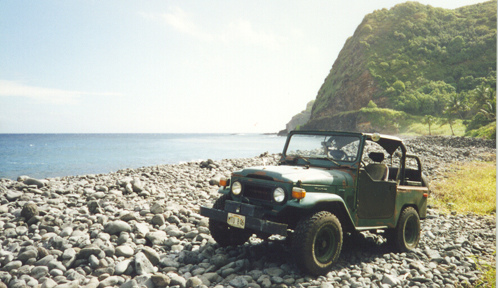
\includegraphics[width=0.48\linewidth]{figSM/2008_001716.jpg} & 
 \\
 \hspace{-2mm}  
\footnotesize{\text{ input image }} &  \\ 
\hspace{-2mm}
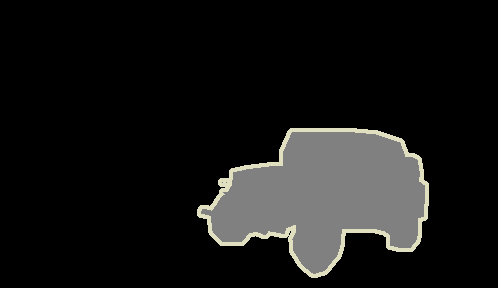
\includegraphics[width=0.48\linewidth]{figSM/2008_001716_gt.png} &
\hspace{-4mm} 
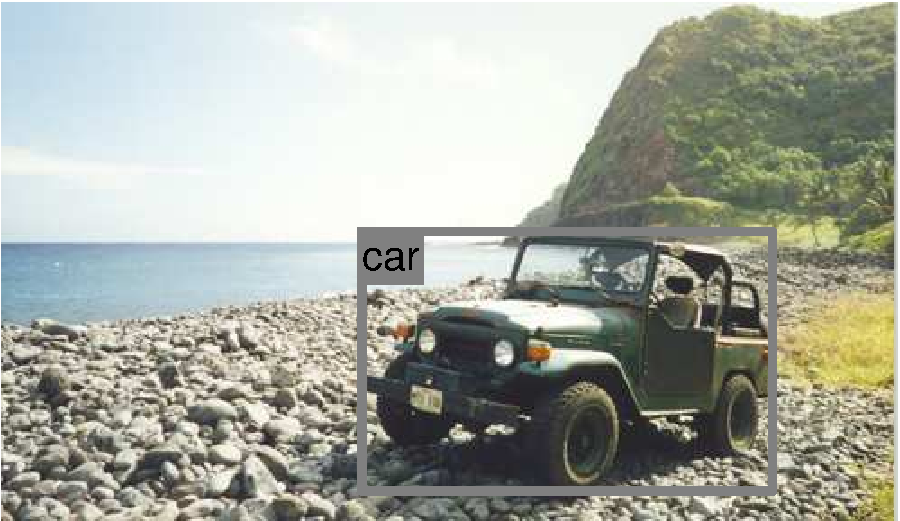
\includegraphics[width=0.48\linewidth]{figSM/2008_001716_bbx-crop.pdf} \\
\hspace{-2mm}  
\footnotesize{\text{(a) full segmentation mask }} & 
 \hspace{-4mm} 
\footnotesize{\text{(b) bounding box}} \\ 
\hspace{-2mm} 
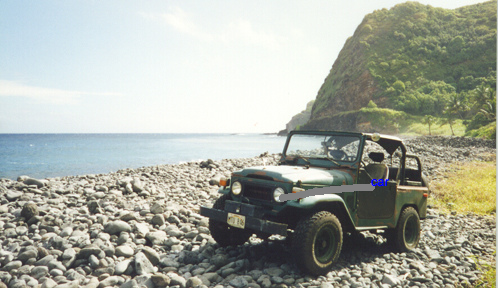
\includegraphics[width=0.48\linewidth]{figSM/2008_001716_anno_15.png} &
\hspace{-4mm} 
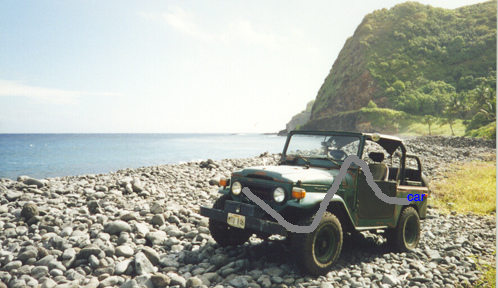
\includegraphics[width=0.48\linewidth]{figSM/2008_001716_anno_3.png}\\
\hspace{-2mm}  
\footnotesize{\text{(c) Semantic Scribbles (Anno-1.5, ours) }} & 
 \hspace{-4mm} 
\footnotesize{\text{(d) Semantic Scribbles (Anno-3, ours)}} \\ 
\end{tabular}$
\caption{A comparison of our annotations to the standard ones used for semantic segmentation. Note that our annotations are significantly cheaper to obtain, but yield comparable results. See the paper for details.}
\label{fig:9}
\end{figure*}



\begin{figure*} 
$\begin{tabular}{ccccc}
\hspace{-2mm}
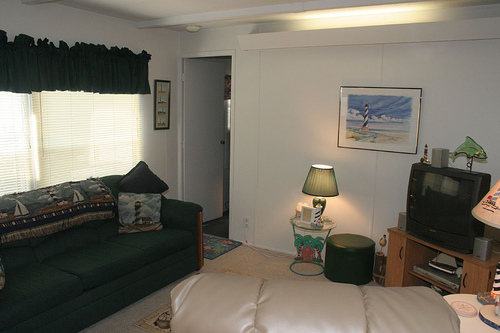
\includegraphics[width=0.48\linewidth]{figSM/2008_001896.jpg} & 
 \\
 \hspace{-2mm}  
\footnotesize{\text{ input image }} &  \\ 
\hspace{-2mm}
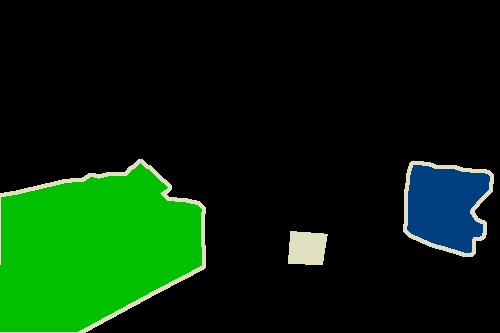
\includegraphics[width=0.48\linewidth]{figSM/2008_001896_gt.png} &
\hspace{-4mm} 
\includegraphics[width=0.48\linewidth]{figSM/2008_001896_bbx-crop.pdf} \\
\hspace{-2mm}  
\footnotesize{\text{(a) full segmentation mask }} & 
 \hspace{-4mm} 
\footnotesize{\text{(b) bounding box}} \\ 
\hspace{-2mm} 
\includegraphics[width=0.48\linewidth]{figSM/2008_001896_anno_15.png} &
\hspace{-4mm} 
\includegraphics[width=0.48\linewidth]{figSM/2008_001896_anno_3.png}\\
\hspace{-2mm}  
\footnotesize{\text{(c) Semantic Scribbles (Anno-1.5, ours) }} & 
 \hspace{-4mm} 
\footnotesize{\text{(d) Semantic Scribbles (Anno-3, ours)}} \\ 
\end{tabular}$
\caption{A comparison of our annotations to the standard ones used for semantic segmentation. Note that our annotations are significantly cheaper to obtain, but yield comparable results. See the paper for details.}
\label{fig:10}
\end{figure*}

\begin{figure*} 
$\begin{tabular}{ccccc}
\hspace{-2mm}
\includegraphics[width=0.48\linewidth]{figSM/2008_001920.jpg} & 
 \\
 \hspace{-2mm}  
\footnotesize{\text{ input image }} &  \\ 
\hspace{-2mm}
\includegraphics[width=0.48\linewidth]{figSM/2008_001920_gt.png} &
\hspace{-4mm} 
\includegraphics[width=0.48\linewidth]{figSM/2008_001920_bbx-crop.pdf} \\
\hspace{-2mm}  
\footnotesize{\text{(a) full segmentation mask }} & 
 \hspace{-4mm} 
\footnotesize{\text{(b) bounding box}} \\ 
\hspace{-2mm} 
\includegraphics[width=0.48\linewidth]{figSM/2008_001920_anno_15.png} &
\hspace{-4mm} 
\includegraphics[width=0.48\linewidth]{figSM/2008_001920_anno_3.png}\\
\hspace{-2mm}  
\footnotesize{\text{(c) Semantic Scribbles (Anno-1.5, ours) }} & 
 \hspace{-4mm} 
\footnotesize{\text{(d) Semantic Scribbles (Anno-3, ours)}} \\ 
\end{tabular}$
\caption{A comparison of our annotations to the standard ones used for semantic segmentation. Note that our annotations are significantly cheaper to obtain, but yield comparable results. See the paper for details.}
\label{fig:11}
\end{figure*}

\begin{figure*} 
$\begin{tabular}{ccccc}
\hspace{-2mm}
\includegraphics[width=0.48\linewidth]{figSM/2008_001997.jpg} & 
 \\
 \hspace{-2mm}  
\footnotesize{\text{ input image }} &  \\ 
\hspace{-2mm}
\includegraphics[width=0.48\linewidth]{figSM/2008_001997_gt.png} &
\hspace{-4mm} 
\includegraphics[width=0.48\linewidth]{figSM/2008_001997_bbx-crop.pdf} \\
\hspace{-2mm}  
\footnotesize{\text{(a) full segmentation mask }} & 
 \hspace{-4mm} 
\footnotesize{\text{(b) bounding box}} \\ 
\hspace{-2mm} 
\includegraphics[width=0.48\linewidth]{figSM/2008_001997_anno_15.png} &
\hspace{-4mm} 
\includegraphics[width=0.48\linewidth]{figSM/2008_001997_anno_3.png}\\
\hspace{-2mm}  
\footnotesize{\text{(c) Semantic Scribbles (Anno-1.5, ours) }} & 
 \hspace{-4mm} 
\footnotesize{\text{(d) Semantic Scribbles (Anno-3, ours)}} \\ 
\end{tabular}$
\caption{A comparison of our annotations to the standard ones used for semantic segmentation. Note that our annotations are significantly cheaper to obtain, but yield comparable results. See the paper for details.}
\label{fig:12}
\end{figure*}


\end{document}


